
%(BEGIN_QUESTION)
% Copyright 2006, Tony R. Kuphaldt, released under the Creative Commons Attribution License (v 1.0)
% This means you may do almost anything with this work of mine, so long as you give me proper credit

The following illustration shows a simple pneumatic ``square-root extractor'' relay mechanism.

$$\includegraphics[width=15.5cm]{i00486x01.eps}$$

As the input pressure increases, the diaphragm expands, pushing the link to the left.  This plugs off the nozzle, increasing the backpressure within the bellows, causing it to expand upward.  As the bellows expands, the nozzle moves up, re-establishing the gap between it and the link's ball-shaped end, until a condition of equilibrium is reached.  The link, of course, will be nearer to level (horizontal) at low input pressure, and more angled (approaching vertical) at high input pressure.

Explain how this angled-link produces the kind of nonlinearity that approximates the square root function.  Also, determine whether this mechanism employs the {\it force-balance} or {\it motion-balance} principle.

\underbar{file i00486}
%(END_QUESTION)





%(BEGIN_ANSWER)

At low input pressures, the link will be nearly horizontal.  At such a shallow angle, the bellows will have to move quite a bit in order to change the link ball/nozzle gap significantly.  This makes the ``gain'' of the system (output/input) rather high at low input pressures, resulting in a graph that is steep at the left end:

$$\includegraphics[width=15.5cm]{i00486x02.eps}$$

Conversely, when the input pressure is higher, the link will be angled more sharply from horizontal.  The steeper this angle, the more vertical motion from the bellows has an effect on link ball/nozzle gap.  Think of it this way: if the link were perfectly vertical (the steepest angle possible), bellows motion would be 100\% effective in changing the gap.  With a perfectly horizontal link, bellows motion has almost no effect on changing the gap.  Thus, as the input pressure increases (and link angle becomes steeper), the ``gain'' of the system decreases.  This results in a transfer function graph that isn't so steep at the right end.

\vskip 10pt

This pneumatic transducer is a real device.  In fact, the Moore Products model 65 transducer uses this very same operating principle to create a ``pseudo'' square root transfer function, used to linearize the output of a differential pressure pneumatic transmitter as it infers flow from the pressure drop across a restriction in a pipe.

This is an example of a {\it motion-balance} mechanism, because the bellows acts as a spring element, converting pressure into a proportional {\it motion}.

%(END_ANSWER)





%(BEGIN_NOTES)


%INDEX% Measurement, flow: pneumatic square root extractor relay

%(END_NOTES)


